\section{Exercises} \vspace{-2mm}

%__________________
\subsection{Inference for a single proportion}

% 1

\eoce{\qt{Vegetarian college students} Suppose that 8\% of college students are vegetarians. Determine if the following statements are true or false, and explain your reasoning.
\begin{parts}
\item The distribution of the sample proportions of vegetarians in random samples of size 60 is approximately normal since $n \ge 30$. 
\item The distribution of the sample proportions of vegetarian college students in random samples of size 50 is right skewed.
\item A random sample of 125 college students where 12\% are vegetarians would be considered unusual. 
\item A random sample of 250 college students where 12\% are vegetarians would be considered unusual.
\item The standard error would be reduced by one-half if we increased the sample size from 125 to~250.
\end{parts}
}{}

% 2

\eoce{\qt{Young Americans, Part I} \label{youngAmericans} About 77\% of young adults think they can achieve the American dream. Determine if the following statements are true or false, and explain your reasoning.\footfullcite{news:youngAmericans1}
\begin{parts}
\item The distribution of sample proportions of young Americans who think they can achieve the American dream in samples of size 20 is left skewed.
\item The distribution of sample proportions of young Americans who think they can achieve the American dream in random samples of size 40 is approximately normal since $n \ge 30$. 
\item A random sample of 60 young Americans where 85\% think they can achieve the American dream would be considered unusual.
\item A random sample of 120 young Americans where 85\% think they can achieve the American dream would be considered unusual.
\end{parts}
}{}

% 3

\eoce{\qt{Orange tabbies} Suppose that 90\% of orange tabby cats are male. Determine if the following statements are true or false, and explain your reasoning.
\begin{parts}
\item The distribution of sample proportions of random samples of size 30 is left skewed.
\item Using a sample size that is 4 times as large will reduce the standard error of the sample proportion by one-half.
\item The distribution of sample proportions of random samples of size 140 is approximately normal.
\item The distribution of sample proportions of random samples of size 280 is approximately normal.
\end{parts}
}{}


% 4

\eoce{\qt{Young Americans, Part II} About 25\% of young Americans have delayed starting a family due to the continued economic slump. Determine if the following statements are true or false, and explain your reasoning.\footfullcite{news:youngAmericans2}
\begin{parts}
\item The distribution of sample proportions of young Americans who have delayed starting a family due to the continued economic slump in random samples of size 12 is right skewed.
\item In order for the distribution of sample proportions of young Americans who have delayed starting a family due to the continued economic slump to be approximately normal, we need random samples where the sample size is at least 40.
\item A random sample of 50 young Americans where 20\% have delayed starting a family due to the continued economic slump would be considered unusual.
\item A random sample of 150 young Americans where 20\% have delayed starting a family due to the continued economic slump would be considered unusual.
\item Tripling the sample size will reduce the standard error of the sample proportion by one-third.
\end{parts}
}{}

% 5

\eoce{\qt{Prop 19 in California} In a 2010 Survey USA poll, 70\% of the 119 respondents between the ages of 18 and 34 said they would vote in the 2010 general election for Prop 19, which would change California law to legalize marijuana and allow it to be regulated and taxed. At a 95\% confidence level, this sample has an 8\% margin of error. Based on this information, determine if the following statements are true or false, and explain your reasoning.\footfullcite{data:prop19_and_offshoreDrill}
\begin{parts}
\item We are 95\% confident that between 62\% and 78\% of the California voters in this sample support Prop 19.
\item We are 95\% confident that between 62\% and 78\% of all California voters between the ages of 18 and 34 support Prop 19.
\item If we considered many random samples of 119 California voters between the ages of 18 and 34, and we calculated 95\% confidence intervals for each, 95\% of them will include the true population proportion of 18-34 year old Californians who support Prop 19.
\item In order to decrease the margin of error to 4\%, we would need to quadruple (multiply by 4) the sample size.
\item Based on this confidence interval, there is sufficient evidence to conclude that a majority of California voters between the ages of 18 and 34 support Prop 19.
\end{parts}
}{}

% 6

\eoce{\qt{2010 Healthcare Law} On June 28, 2012 the U.S. Supreme Court upheld the much debated 2010 healthcare law, declaring it constitutional. A Gallup poll released the day after this decision indicates that 46\% of 1,012 Americans agree with this decision. At a 95\% confidence level, this sample has a 3\% margin of error. Based on this information, determine if the following statements are true or false, and explain your reasoning.\footfullcite{data:healthcare2010}
\begin{parts}
\item We are 95\% confident that between  43\% and 49\% of Americans in this sample support the decision of the U.S. Supreme Court on the 2010 healthcare law.
\item We are 95\% confident that between 43\% and 49\% of Americans support the decision of the U.S. Supreme Court on the 2010 healthcare law.
\item If we considered many random samples of 1,012 Americans, and we calculated the sample proportions of those who support the decision of the U.S. Supreme Court, 95\% of those sample proportions will be between  43\% and 49\%.
\item The margin of error at a 90\% confidence level would be higher than 3\%.
\end{parts}
}{}

% 7

\eoce{\qt{Fireworks on July $4^{\text{th}}$} In late June 2012, Survey USA published results of a survey stating that 56\% of the 600 randomly sampled Kansas residents planned to set off fireworks on July~$4^{th}$. Determine the margin of error for the 56\% point estimate using a 95\% confidence level.\footfullcite{data:july4}
}{}

% 8

\eoce{\qt{Elderly drivers} In January 2011, The Marist Poll published a report stating that 66\% of adults nationally think licensed drivers should be required to retake their road test once they reach 65 years of age. It was also reported that interviews were conducted on 1,018 American adults, and that the margin of error was 3\% using a 95\% confidence level. \footfullcite{data:elderlyDriving}
\begin{parts}
\item Verify the margin of error reported by The Marist Poll. 
\item Based on a 95\% confidence interval, does the poll provide convincing evidence that \textit{more than} 70\% of the population think that licensed drivers should be required to retake their road test once they turn 65?
\end{parts}
}{}


\textC{\pagebreak}

% 9

\eoce{\qt{Life after college} We are interested in estimating the proportion of graduates at a mid-sized university who found a job within one year of completing their undergraduate degree. Suppose we conduct a survey and find out that 348 of the 400 randomly sampled graduates found jobs. The graduating class under consideration included over 4500 students.
\begin{parts}
\item Describe the population parameter of interest. What is the value of the point estimate of this parameter?
\item Check if the conditions for constructing a confidence interval based on these data are met.
\item Calculate a 95\% confidence interval for the proportion of graduates who found a job within one year of completing their undergraduate degree at this university, and interpret it in the context of the data.
\item What does ``95\% confidence" mean?
\item Now calculate a 99\% confidence interval for the same parameter and interpret it in the context of the data.
\item Compare the widths of the 95\% and 99\% confidence intervals. Which one is wider? Explain.
\end{parts}
}{}

% 10

\eoce{\qt{Life rating in Greece} Greece has faced a severe economic crisis since the end of 2009. A Gallup poll surveyed 1,000 randomly sampled Greeks in 2011 and found that 25\% of them said they would rate their lives poorly enough to be considered ``suffering''.\footfullcite{data:suffering}
\begin{parts}
\item Describe the population parameter of interest. What is the value of the point estimate of this parameter?
\item Check if the conditions required for constructing a confidence interval based on these data are met.
\item Construct a 95\% confidence interval for the proportion of Greeks who are ``suffering".
\item Without doing any calculations, describe what would happen to the confidence interval if we decided to use a higher confidence level.
\item Without doing any calculations, describe what would happen to the confidence interval if we used a larger sample.
\end{parts}
}{}

% 11

\eoce{\qt{Study abroad} A survey on 1,509 high school seniors who took the SAT and who completed an optional web survey between April 25 and April 30, 2007 shows that 55\% of high school seniors are fairly certain that they will participate in a study abroad program in college.\footfullcite{data:studyAbroad}
\begin{parts}
\item Is this sample a representative sample from the population of all high school seniors in the US? Explain your reasoning.
\item Let's suppose the conditions for inference are met. Even if your answer to part (a) indicated that this approach would not be reliable, this analysis may still be interesting to carry out (though not report). Construct a 90\% confidence interval for the proportion of high school seniors (of those who took the SAT) who are fairly certain they will participate in a study abroad program in college, and interpret this interval in context.
\item What does ``90\% confidence" mean?
\item Based on this interval, would it be appropriate to claim that the majority of high school seniors are fairly certain that they will participate in a study abroad program in college?
\end{parts}
}{}


\textC{\pagebreak}

% 12

\eoce{\qt{Legalization of marijuana, Part I} \label{legalizeMarijuana} The 2010 General Social Survey asked 1,259 US residents: ``Do you think the use of marijuana should be made legal, or not?" 48\% of the respondents said it should be made legal.\footfullcite{data:gss:2010}
\begin{parts}
\item Is 48\% a sample statistic or a population parameter? Explain.
\item Construct a 95\% confidence interval for the proportion of US residents who think marijuana should be made legal, and interpret it in the context of the data.
\item A critic points out that this 95\% confidence interval is only accurate if the statistic follows a normal distribution, or if the normal model is a good approximation. Is this true for these data? Explain.
\item A news piece on this survey's findings states, ``Majority of Americans think marijuana should be legalized.'' Based on your confidence interval, is this news piece's statement justified? 
\end{parts}
}{}

% 13

\eoce{\qt{Public option, Part I} \label{publicOption} A \textit{Washington Post} article from 2009 reported that ``support for a government-run health-care plan to compete with private insurers has rebounded from its summertime lows and wins clear majority support from the public." More specifically, the article says ``seven in 10 Democrats back the plan, while almost nine in 10 Republicans oppose it. Independents divide 52 percent against, 42 percent in favor of the legislation." (6\% responded with ``other".) There were 819 Democrats, 566 Republicans and 783 Independents surveyed. \footfullcite{news:publicOption}
\begin{parts}
\item A political pundit on TV claims that a majority of Independents oppose the health care public option plan. Do these data provide strong evidence to support this statement?
\item Would you expect a confidence interval for the proportion of Independents who oppose the public option plan to include 0.5? Explain.
\end{parts}
}{}

% 14

\eoce{\qt{The Civil War} A national survey conducted in 2011 among a simple random sample of 1,507 adults shows that 56\% of Americans think the Civil War is still relevant to American politics and political life. \footfullcite{data:civilWar} 
\begin{parts}
\item Conduct a hypothesis test to determine if these data provide strong evidence that the majority of the Americans think the Civil War is still relevant.
\item Interpret the p-value in this context.
\item Calculate a 90\% confidence interval for the proportion of Americans who think the Civil War is still relevant. Interpret the interval in this context, and comment on whether or not the confidence interval agrees with the conclusion of the hypothesis test.
\end{parts}
}{}

% 15

\eoce{\qt{Browsing on the mobile device} A 2012 survey of  2,254 American adults indicates that 17\% of cell phone owners do their browsing on their phone rather than a computer or other device.\footfullcite{data:mobileBrowse}
\begin{parts}
\item  According to an online article, a report from a mobile research company indicates that 38 percent of Chinese mobile web users only access the internet through their cell phones.\footfullcite{news:mobileBrowseChinese} Conduct a hypothesis test to determine if these data provide strong evidence that the proportion of Americans who only use their cell phones to access the internet is different than the Chinese proportion of 38\%.
\item Interpret the p-value in this context.
\item Calculate a 95\% confidence interval for the proportion of Americans who access the internet on their cell phones, and interpret the interval in this context.
\end{parts}
}{}


% 16

\eoce{\qt{Is college worth it? Part I} \label{collegeWorthIt} Among a simple random sample of 331 American adults who do not have a four-year college degree and are not currently enrolled in school, 48\% said they decided not to go to college because they could not afford school. \footfullcite{data:collegeWorthIt}
\begin{parts}
\item A newspaper article states that only a minority of the Americans who decide not to go to college do so because they cannot afford it and uses the point estimate from this survey as evidence. Conduct a hypothesis test to determine if these data provide strong evidence supporting this statement.
\item Would you expect a confidence interval for the proportion of American adults who decide not to go to college because they cannot afford it to include 0.5? Explain.
\end{parts}
}{}

% 17

\eoce{\qt{Taste test} \label{sodaDietReg} Some people claim that they can tell the difference between a diet soda and a regular soda in the first sip. A researcher wanting to test this claim randomly sampled 80 such people. He then filled 80 plain white cups with soda, half diet and half regular through random assignment, and asked each person to take one sip from their cup and identify the soda as diet or regular. 53 participants correctly identified the soda.
\begin{parts}
\item Do these data provide strong evidence that these people are able to detect the difference between diet and regular soda, in other words, are the results significantly better than just random guessing?
\item Interpret the p-value in this context.
\end{parts}
}{}

% 18

\eoce{\qt{Is college worth it? Part II} Exercise~\ref{collegeWorthIt} presents the results of a poll where 48\% of 331 Americans who decide to not go to college do so because they cannot afford it.
\begin{parts}
\item Calculate a 90\% confidence interval for the proportion of Americans who decide to not go to college because they cannot afford it, and interpret the interval in context.
\item Suppose we wanted the margin of error for the 90\% confidence level to be about 1.5\%. How large of a survey would you recommend?
\end{parts}
}{}

% 19

\eoce{\qt{College smokers} \label{UnivSmoke} We are interested in estimating the proportion of students at a university who smoke. Out of a random sample of 200 students from this university, 40 students smoke.
\begin{parts}
\item Calculate a 95\% confidence interval for the proportion of students at this university who smoke, and interpret this interval in context. (Reminder: check conditions)
\item If we wanted the margin of error to be no larger than 2\% at a 95\% confidence level for the proportion of students who smoke, how big of a sample would we need? 
\end{parts}
}{}

% 20

\eoce{\qt{Legalize Marijuana, Part II} As discussed in Exercise~\ref{legalizeMarijuana}, the 2010 General Social Survey reported a sample where about 48\% of US residents thought marijuana should be made legal. If we wanted to limit the margin of error of a 95\% confidence interval to 2\%, about how many Americans would we need to survey ?
}{}

% 21

\eoce{\qt{Public option, Part II} Exercise~\ref{publicOption} presents the results of a poll evaluating support for the health care public option in 2009, reporting that 52\% of Independents in the sample opposed the public option. If we wanted to estimate this number to within 1\% with 90\% confidence, what would be an appropriate sample size?
}{}

\textC{\newpage}

% 22

\eoce{\qt{Acetaminophen and liver damage} It is believed that large doses of acetaminophen (the active ingredient in over the counter pain relievers like Tylenol) may cause damage to the liver. A researcher wants to conduct a study to estimate the proportion of acetaminophen users who have liver damage. For participating in this study, he will pay each subject \$20 and provide a free medical consultation if the patient has liver damage.
\begin{parts}
\item If he wants to limit the margin of error of his 98\% confidence interval to 2\%, what is the minimum amount of money he needs to set aside to pay his subjects?
\item The amount you calculated in part (a) is substantially over his budget so he decides to use fewer subjects. How will this affect the width of his confidence interval?
\end{parts}
}{}


%__________________
\subsection{Difference of two proportions}

% 23

\eoce{\qt{Social experiment, Part I} \label{socExp} A ``social experiment" conducted by a TV program questioned what people do when they see a very obviously bruised woman getting picked on by her boyfriend. On two different occasions at the same restaurant, the same couple was depicted. In one scenario the woman was dressed ``provocatively'' and in the other scenario the woman was dressed ``conservatively''. The table below shows how many restaurant diners were present under each scenario, and whether or not they intervened.
\begin{center}
\begin{tabular}{ll cc c} 
			&				& \multicolumn{2}{c}{\textit{Scenario}} \\
\cline{3-4}
							&			& Provocative	& Conservative 	& Total	\\
\cline{2-5}
\multirow{2}{*}{\textit{Intervene}}	&Yes 		& 5	 	& 15		& 20 	\\
							&No			& 15	 	& 10 	 	& 25 \\
\cline{2-5}
							&Total		& 20		& 25		& 45 \\
\end{tabular}
\end{center}
Explain why the sampling distribution of the difference between the proportions of interventions under provocative and conservative scenarios does not follow an approximately normal distribution.
}{}

% 24

\eoce{\qt{Heart transplant success} The Stanford University Heart Transplant Study was conducted to determine whether an experimental heart transplant program increased lifespan. Each patient entering the program was officially designated a heart transplant candidate, meaning that he was gravely ill and might benefit from a new heart. Patients were randomly assigned into treatment and control groups. Patients in the treatment group received a transplant, and those in the control group did not. The table below displays how many patients survived and died in each group. \footfullcite{Turnbull+Brown+Hu:1974}\vspace{-2mm}
\begin{center}
\begin{tabular}{rcc}
  \hline
 & control & treatment \\ 
  \hline
alive &   4 &  24 \\ 
  dead &  30 &  45 \\ 
   \hline
\end{tabular}
\end{center}
A hypothesis test would reject the conclusion that the survival rate is the same in each group, and so we might like to calculate a confidence interval. Explain why we cannot construct such an interval using the normal approximation. What might go wrong if we constructed the confidence interval despite this problem?
}{}

\textC{\newpage}

% 25

\eoce{\qt{Gender and color preference} A 2001 study asked 1,924 male and 3,666 female undergraduate college students their favorite color. A 95\% confidence interval for the difference between the proportions of males and females whose favorite color is black $(p_{male} - p_{female})$ was calculated to be (0.02, 0.06). Based on this information, determine if the following statements are true or false, and explain your reasoning for each statement you identify as false.\footfullcite{Ellis:2001}
\begin{parts}
\item We are 95\% confident that the true proportion of males whose favorite color is black is 2\% lower to 6\% higher than the true proportion of females whose favorite color is black.
\item We are 95\% confident that the true proportion of males whose favorite color is black is 2\% to 6\% higher than the true proportion of females whose favorite color is black.
\item 95\% of random samples will produce 95\% confidence intervals that include the true difference between the population proportions of males and females whose favorite color is black.
\item We can conclude that there is a significant difference between the proportions of males and females whose favorite color is black and that the difference between the two sample proportions is too large to plausibly be due to chance.
\item The 95\% confidence interval for $(p_{female} - p_{male})$ cannot be calculated with only the information given in this exercise.
\end{parts}
}{}

% 26

\eoce{\qt{The Daily Show} A 2010 Pew Research foundation poll indicates that among 1,099 college graduates, 33\% watch The Daily Show. Meanwhile, 22\% of the 1,110 people with a high school degree but no college degree in the poll watch The Daily Show. A 95\% confidence interval for $(p_\text{college grad} - p_\text{HS or less})$, where $p$ is the proportion of those who watch The Daily Show, is (0.07, 0.15). Based on this information, determine if the following statements are true or false, and explain your reasoning if you identify the statement as false.\footfullcite{data:dailyShow}
\begin{parts}
\item At the 5\% significance level, the data provide convincing evidence of a difference between the proportions of college graduates and those with a high school degree or less who watch The Daily Show.
\item We are 95\% confident that 7\% less to 15\% more college graduates watch The Daily Show than those with a high school degree or less.
\item 95\% of random samples of 1,099 college graduates and 1,110 people with a high school degree or less will yield differences in sample proportions between 7\% and 15\%.
\item A 90\% confidence interval for $(p_\text{college grad} - p_\text{HS or less})$ would be wider.
\item A 95\% confidence interval for $(p_\text{HS or less} - p_\text{college grad})$ is (-0.15,-0.07).
\end{parts}
}{}

% 27

\eoce{\qt{Public Option, Part III} Exercise~\ref{publicOption} presents the results of a poll evaluating support for the health care public option plan in 2009. 70\% of 819 Democrats and 42\% of 783 Independents support the public option.
\begin{parts}
\item Calculate a 95\% confidence interval for the difference between $(p_{D} - p_{I})$ and interpret it in this context. We have already checked conditions for you.
\item True or false: If we had picked a random Democrat and a random Independent at the time of this poll, it is more likely that the Democrat would support the public option than the Independent.
\end{parts}
}{}

\textC{\pagebreak}

% 28

\eoce{\qt{Sleep deprivation, CA vs. OR, Part I} \label{OregonCaliSleepCI} According to a report on sleep deprivation by the Centers for Disease Control and Prevention, the proportion of California residents who reported insufficient rest or sleep during each of the preceding 30 days is 8.0\%, while this proportion is 8.8\% for Oregon residents. These data are based on simple random samples of 11,545 California and 4,691 Oregon residents. Calculate a 95\% confidence interval for the difference between the proportions of Californians and Oregonians who are sleep deprived and interpret it in context of the data.\footfullcite{data:sleepCAandOR}
}{}

% 29

\eoce{\qt{Offshore drilling, Part I} \label{drillBabyDrill} A 2010 survey asked 827 randomly sampled registered voters in California ``Do you support? Or do you oppose? Drilling for oil and natural gas off the Coast of California? Or do you not know enough to say?" Below is the distribution of responses, separated based on whether or not the respondent graduated from college. \footfullcite{data:prop19_and_offshoreDrill} \\[1.3mm]
\noindent\begin{minipage}[c]{0.6\textwidth}
\begin{parts}
\item What percent of college graduates and what percent of the non-college graduates in this sample do not know enough to have an opinion on drilling for oil and natural gas off the Coast of California?
\item Conduct a hypothesis test to determine if the data provide strong evidence that the proportion of college graduates who do not have an opinion on this issue is different than that of non-college graduates.
\end{parts}
\end{minipage}
\begin{minipage}[c]{0.4\textwidth}
\begin{center}
\begin{tabular}{l c c}
				& \multicolumn{2}{c}{\textit{College Grad}} \\
\cline{2-3}
						& Yes		& No				\\
\cline{1-3}
Support		& 154		& 132			\\
Oppose		& 180		& 126			\\
Do not know	& 104		& 131			\\
\cline{1-3}
 Total		& 438		& 389		
\end{tabular}
\end{center}
\end{minipage}
}{}


% 30

\eoce{\qt{Sleep deprivation, CA vs. OR, Part II} Exercise~\ref{OregonCaliSleepCI} provides data on sleep deprivation rates of Californians and Oregonians. The proportion of California residents who reported insufficient rest or sleep during each of the preceding 30 days is 8.0\%, while this proportion is 8.8\% for Oregon residents. These data are based on simple random samples of 11,545 California and 4,691 Oregon residents. 
\begin{parts}
\item Conduct a hypothesis test to determine if these data provide strong evidence the rate of sleep deprivation is different for the two states. (Reminder: check conditions)
\item It is possible the conclusion of the test in part (a) is incorrect. If this is the case, what type of error was made?
\end{parts}
}{}

% 31

\eoce{\qt{Offshore drilling, Part II} Results of a poll evaluating support for drilling for oil and natural gas off the coast of California were introduced in Exercise~\ref{drillBabyDrill}.
\begin{center}
\begin{tabular}{l c c}
				& \multicolumn{2}{c}{\textit{College Grad}} \\
\cline{2-3}
						& Yes		& No				\\
\cline{1-3}
Support		& 154		& 132			\\
Oppose		& 180		& 126			\\
Do not know	& 104		& 131			\\
\cline{1-3}
 Total		& 438		& 389		
\end{tabular}
\end{center}

\begin{parts}
\item What percent of college graduates and what percent of the non-college graduates in this sample support drilling for oil and natural gas off the Coast of California?
\item Conduct a hypothesis test to determine if the data provide strong evidence that the proportion of college graduates who support off-shore drilling in California is different than that of non-college graduates.
\end{parts}
}{}

\textC{\newpage}

% 32

\eoce{\qt{Full body scan, Part I} \label{fullBodyScan} A news article reports that ``Americans have differing views on two potentially inconvenient and invasive practices that airports could implement to uncover potential terrorist attacks." This news piece was based on a survey conducted among a random sample of 1,137 adults nationwide, interviewed by telephone November 7-10, 2010, where one of the questions on the survey was ``Some airports are now using `full-body' digital x-ray machines to electronically screen passengers in airport security lines. Do you think these new x-ray machines should or should not be used at airports?" Below is a summary of responses based on party affiliation. \footfullcite{news:fullBodyScan}
\begin{center}
\begin{tabular}{ll  cc c} 
			&				& \multicolumn{3}{c}{\textit{Party Affiliation}} \\
\cline{3-5}
							&					& Republican 	& Democrat 	& Independent	\\
\cline{2-5}
\multirow{3}{*}{\textit{Answer}}		&Should				& 264	 	& 299		& 351 	\\
							&Should not			& 38	 		& 55 	 		& 77 \\
							&Don't know/No answer	& 16	 		& 15 	 		& 22 \\
\cline{2-5}
							&Total				& 318		& 369		& 450
\end{tabular}
\end{center}

\begin{parts}
\item Conduct an appropriate hypothesis test evaluating whether there is a difference in the proportion of Republicans and Democrats who think the full-body scans should be applied in airports. Assume that all relevant conditions are met.
\item The conclusion of the test in part (a) may be incorrect, meaning a testing error was made. If an error was made, was it a Type~1 or a Type~2 Error? Explain.
\end{parts}
}{}


% 33

\eoce{\qt{Sleep deprived transportation workers} The National Sleep Foundation conducted a survey on the sleep habits of randomly sampled transportation workers and a control sample of non-transportation workers. The results of the survey are shown below.\footfullcite{data:sleepTransport}\vspace{-1.8mm}
\begin{center}
\begin{tabular}{l c c c c c }
						& 			& \multicolumn{4}{c}{\textit{Transportation Professionals}} \\
\cline{3-6}
						& 			& 		& Truck	& Train		& Bux/Taxi/Limo		\\
						& \textit{Control}& Pilots	& Drivers	& Operators	& Drivers				 \\
\cline{1-6}
Less than 6 hours of sleep	& 35			& 19		& 35		& 29			& 21				 	\\
6 to 8 hours of sleep			& 193		& 132	& 117	& 119		& 131				\\
More than 8 hours			& 64			& 51		& 51		& 32			& 58					\\
\cline{1-6}
Total						& 292		& 202	& 203	& 180		& 210		
\end{tabular}
\end{center}\vspace{-1.2mm}
Conduct a hypothesis test to evaluate if these data provide evidence of a difference between the proportions of truck drivers and non-transportation workers (the control group) who get less than 6 hours of sleep per day, i.e. are considered sleep deprived.
}{}

\textC{\newpage}

% 34

\eoce{\qt{Prenatal vitamins and Autism} Researchers studying the link between prenatal vitamin use and autism surveyed the mothers of a random sample of children aged 24 - 60 months with autism and conducted another separate random sample for children with typical development. The table below shows the number of mothers in each group who did and did not use prenatal vitamins during the three months before pregnancy (periconceptional period).\footfullcite{Schmidt:2011}\vspace{-1.8mm}
\begin{center}
\begin{tabular}{l l c c c}
								&			& \multicolumn{2}{c}{\textit{Autism}}	&		\\
\cline{3-4}
								&			& Autism		& Typical development		& Total	\\
\cline{2-5}
\textit{Periconceptional}				& No vitamin			& 111		& 70						& 181	\\
\textit{prenatal vitamin}				& Vitamin		& 143		& 159					& 302	\\
\cline{2-5}
								& Total		& 254		& 229					& 483
\end{tabular}
\end{center}\vspace{-4.2mm}
\begin{parts}
\item State appropriate hypotheses to test for independence of use of prenatal vitamins during the three months before pregnancy and autism.
\item Complete the hypothesis test and state an appropriate conclusion. (Reminder: verify any necessary conditions for the test.)
\item A New York Times article reporting on this study was titled ``Prenatal Vitamins May Ward Off Autism". Do you find the title of this article to be appropriate? Explain your answer. Additionally, propose an alternative title.\footfullcite{news:prenatalVitAutism}
\end{parts}
}{}

% 35

\eoce{\qt{HIV in sub-Saharan Africa} In July 2008 the US National Institutes of Health announced that it was stopping a clinical study early because of unexpected results. The study population consisted of HIV-infected women in sub-Saharan Africa who had been given single dose Nevaripine (a treatment for HIV) while giving birth, to prevent transmission of HIV to the infant.  The study was a randomized comparison of continued treatment of a woman (after successful childbirth) with Nevaripine vs. Lopinavir, a second drug used to treat HIV. 240 women participated in the study; 120 were randomized to each of the two treatments. Twenty-four weeks after starting the study treatment, each woman was tested to determine if the HIV infection was becoming worse (an outcome called \textit{virologic failure}). Twenty-six of the 120 women treated with Nevaripine experienced virologic failure, while 10 of the 120 women treated with the other drug experienced virologic failure. \footfullcite{Lockman:2007}
\begin{parts}
\item Create a two-way table presenting the results of this study.
\item State appropriate hypotheses to test for independence of treatment and virologic failure.
\item Complete the hypothesis test and state an appropriate conclusion. (Reminder: verify any necessary conditions for the test.)
\end{parts}
}{}

% 36

\eoce{\qt{Diabetes and unemployment} A 2012 Gallup poll surveyed Americans about their employment status and whether or not they have diabetes. The survey results indicate that 1.5\% of the 47,774 employed (full or part time) and 2.5\% of the 5,855 unemployed 18-29 year olds have diabetes.\footfullcite{data:employmentDiabetes}
\begin{parts}
\item Create a two-way table presenting the results of this study.
\item State appropriate hypotheses to test for independence of incidence of diabetes and employment status.
\item The sample difference is about 1\%. If we completed the hypothesis test, we would find that the p-value is very small (about 0), meaning the difference is statistically significant. Use this result to explain the difference between statistically significant and practically significant findings.
\end{parts}
}{}

% 37

\eoce{\qt{Active learning} A teacher wanting to increase the active learning component of her course is concerned about student reactions to changes she is planning to make. She conducts a survey in her class, asking students whether they believe more active learning in the classroom (hands on exercises) instead of traditional lecture will helps improve their learning. She does this at the beginning and end of the semester and wants to evaluate whether students' opinions have changed over the semester. Can she used the methods we learned in this chapter for this analysis? Explain your reasoning.
}{}

% 38

\eoce{\qt{An apple a day keeps the doctor away} A physical education teacher at a high school wanting to increase awareness on issues of nutrition and health asked her students at the beginning of the semester whether they believed the expression ``an apple a day keeps the doctor away", and 40\% of the students responded yes. Throughout the semester she started each class with a brief discussion of a study highlighting positive effects of eating more fruits and vegetables. She conducted the same apple-a-day survey at the end of the semester, and this time 60\% of the students responded yes. Can she used the methods we learned in this chapter for this analysis? Explain your reasoning.
}{}

%%%%%%%%%%%%%%%%%%%%%%

\subsection{Testing for goodness of fit using chi-square}

%%%%%%%%%%%%%%%%%%%%%%

% 39

\eoce{\qt{True or false, Part I} Determine if the statements below are true or false. For each false statement, suggest an alternative wording to make it a true statement.
\begin{parts}
\item The chi-square distribution, just like the normal distribution, has two parameters, mean and standard deviation.
\item The chi-square distribution is always right skewed, regardless of the value of the degrees of freedom parameter.
\item The chi-square statistic is always positive.
\item As the degrees of freedom increases, the shape of the chi-square distribution becomes more skewed.
\end{parts}
}{}

% 40

\eoce{\qt{True or false, Part II} Determine if the statements below are true or false. For each false statement, suggest an alternative wording to make it a true statement.
\begin{parts}
\item As the degrees of freedom increases, the mean of the chi-square distribution increases.
\item If you found $X^2 = 10$ with $df = 5$ you would fail to reject $H_0$ at the 5\% significance level.
\item When finding the p-value of a chi-square test, we always shade the tail areas in both tails.
\item As the degrees of freedom increases, the variability of the chi-square distribution decreases.
\end{parts}
}{}

% 41

\eoce{\qt{Open source textbook} A professor using an open source introductory statistics book predicts that 60\% of the students will purchase a hard copy of the book, 25\% will print it out from the web, and 15\% will read it online. At the end of the semester he asks his students to complete a survey where they indicate what format of the book they used. Of the 126 students, 71 said they bought a hard copy of the book, 30 said they printed it out from the web, and 25 said they read it online.
\begin{parts}
\item State the hypotheses for testing if the professor's predictions were inaccurate.
\item How many students did the professor expect to buy the book, print the book, and read the book exclusively online?
\item This is an appropriate setting for a chi-square test. List the conditions required for a test and verify they are satisfied.
\item Calculate the chi-squared statistic, the degrees of freedom associated with it, and the p-value.
\item Based on the p-value calculated in part (d), what is the conclusion of the hypothesis test? Interpret your conclusion in this context.
\end{parts}
}{}

% 42

\eoce{\qt{Evolution vs. creationism} A Gallup Poll released in December 2010 asked 1019 adults living in the Continental U.S. about their belief in the origin of humans. These results, along with results from a more comprehensive poll from 2001 (that we will assume to be exactly accurate), are summarized in the table below: \footfullcite{CreationismGallup}
\begin{center}
\begin{tabular}{l c c}
	& \multicolumn{2}{c}{\textit{Year}} \\
\cline{2-3}
\textit{Response}								& 2010	& 2001 \\
\hline
Humans evolved, with God guiding (1)				& 38\% 	& 37\% \\
Humans evolved, but God had no part in process (2) 	& 16\% 	& 12\% \\
God created humans  in present form (3) 				& 40\% 	& 45\% \\
Other / No opinion (4)							& 6\% 	& 6\% \\
\hline
\end{tabular}
\end{center} 

\begin{parts}
\item Calculate the actual number of respondents in 2010 that fall in each response category.
\item State hypotheses for the following research question: have beliefs on the origin of human life changed since 2001?
\item Calculate the expected number of respondents in each category under the condition that the null hypothesis from part~(b) is true.
\item Conduct a chi-square test and state your conclusion. (Reminder: verify conditions.)
\end{parts}
}{}

% 43

\eoce{\qt{Rock-paper-scissors} Rock-paper-scissors is a hand game played by two or more people where players choose to sign either �rock�, �paper�, or �scissors� with their hands. For your AP Statistics class project, you want to evaluate whether players choose between these three options randomly, or if certain options are favored above others. You ask two friends to play rock-paper-scissors and count the times each option is played. The following table summarizes the data:
\begin{center}
\begin{tabular}{c c c}
Rock		& Paper	& Scissors 	 \\
\hline
43		& 21		& 35	
\end{tabular}
\end{center}
Use these data to evaluate whether players choose between these three options randomly, or if certain options are favored above others. Make sure to clearly outline each step of your analysis, and interpret your results in context of the data and the research question.
}{}

% 44

\eoce{\qt{Barking deer} Microhabitat factors associated with forage and bed sites of barking deer in Hainan Island, China were examined from 2001 to 2002. In this region woods make up 4.8\% of the land, cultivated grass plot makes up 14.7\% and deciduous forests makes up 39.6\%. Of the 426 sites where the deer forage, 4 were categorized as woods, 16 as cultivated grassplot, and 61 as deciduous forests. The table below summarizes these data.\footfullcite{Teng:2004}
\begin{center}
\begin{tabular}{c c c c c}
Woods	& Cultivated grassplot	& Deciduous forests	& Other	 & Total \\
\hline
4		& 16					& 67			& 345	& 426 \\
\end{tabular}
\end{center}

\noindent \begin{minipage}[c]{0.7\textwidth}
\begin{parts}
\item Write the hypotheses for testing if barking deer prefer to forage in certain habitats over others.
\item What type of test can we use to answer this research question?
\item Check if the assumptions and conditions required for this test are satisfied.
\item Do these data provide convincing evidence that barking deer prefer to forage in certain habitats over others? Conduct an appropriate hypothesis test to answer this research question.
\end{parts}
\end{minipage}
\begin{minipage}[c]{0.03\textwidth}
$\:$ \\
\end{minipage}
\begin{minipage}[c]{0.28\textwidth}
\begin{center}
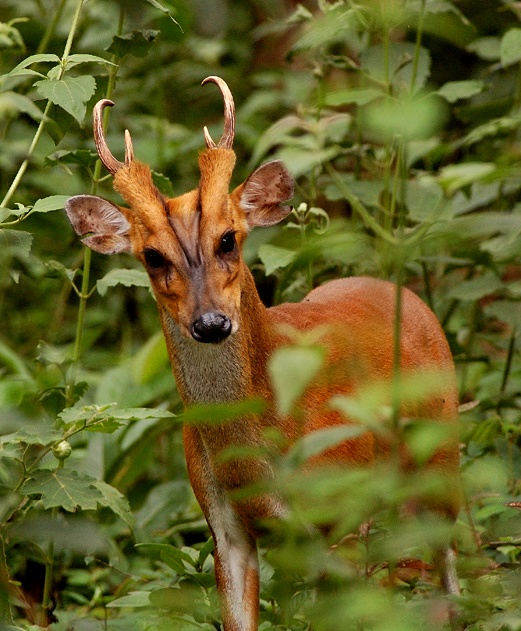
\includegraphics[width=0.7\textwidth]{ch_inference_for_props/figures/eoce/images/barking_deer} \\
{\footnotesize Photo by Shrikant Rao (\oiRedirect{textbook-flickr_shrikant_rao_barking_deer}{http://flic.kr/p/4Xjdkk}) \oiRedirect{textbook-CC_BY_2}{CC~BY~2.0~license}}
\end{center}
\end{minipage}
}{}

%__________________
\subsection{Testing for independence in two-way tables}

% 45

\eoce{\qt{Quitters} Does being part of a support group affect the ability of people to quit smoking? A county health department enrolled 300 smokers in a randomized experiment. 150 participants were assigned to a group that used a nicotine patch and met weekly with a support group; the other 150 received the patch and did not meet with a support group. At the end of the study, 40 of the participants in the patch plus support group had quit smoking while only 30 smokers had  quit in the other group.

\begin{parts}
\item Create a two-way table presenting the results of this study.
\item Answer each of the following questions under the null hypothesis that being part of a support group does not affect the ability of people to quit smoking, and indicate whether the expected values are higher or lower than the observed values.
\begin{subparts}
\item How many subjects in the ``patch + support" group would you expect to quit?
\item How many subjects in the ``patch only" group would you expect to not quit?
\end{subparts}
\end{parts}
}{}

% 46

\eoce{\qt{Full body scan, Part II} The table below summarizes a data set we first encountered in Exercise~\ref{fullBodyScan} regarding views on full-body scans and political affiliation. The differences in each political group may be due to chance. Complete the following computations under the null hypothesis of independence between an individual's party affiliation and his support of full-body scans. It may be useful to first add on an extra column for row totals before proceeding with the computations.
\begin{center}
\begin{tabular}{ll  cc c} 
			&				& \multicolumn{3}{c}{\textit{Party Affiliation}} \\
\cline{3-5}
							&					& Republican 	& Democrat 	& Independent	\\
\cline{2-5}
\multirow{3}{*}{\textit{Answer}}		&Should				& 264	 	& 299		& 351 	\\
							&Should not			& 38	 		& 55 	 		& 77 \\
							&Don't know/No answer	& 16	 		& 15 	 		& 22 \\
\cline{2-5}
							&Total				& 318		& 369		& 450
\end{tabular}
\end{center}

\begin{parts}
\item How many Republicans would you expect to not support the use of full-body scans?
\item How many Democrats would you expect to support the use of full-body scans?
\item How many Independents would you expect to not know or not answer?
\end{parts}
}{}

% 47

\eoce{\qt{Offshore drilling, Part III} The table below summarizes a data set we first encountered in Exercise~\ref{drillBabyDrill} that examines the responses of a random sample of college graduates and non-graduates on the topic of oil drilling. Complete a chi-square test for these data to check whether there is a statistically significant difference in responses from college graduates and non-graduates.
\begin{center}
\begin{tabular}{l c c}
			& \multicolumn{2}{c}{\textit{College Grad}} \\
\cline{2-3}
			& Yes		& No				\\
\cline{1-3}
Support		& 154		& 132			\\
Oppose		& 180		& 126			\\
Do not know	& 104		& 131			\\
\cline{1-3}
 Total		& 438		& 389		
\end{tabular}
\end{center}
}{}

\textC{\newpage}

% 48

\eoce{\qt{Coffee and Depression} Researchers conducted a study investigating the relationship between caffeinated coffee consumption and risk of depression in women. They collected data on 50,739 women free of depression symptoms at the start of the study in the year 1996, and these women were followed through 2006. The researchers used questionnaires to collect data on caffeinated coffee consumption, asked each individual about physician-diagnosed depression, and also asked about the use of antidepressants. The table below shows the distribution of incidences of depression by amount of caffeinated coffee consumption.\footfullcite{Lucas:2011}

\begin{adjustwidth}{-4em}{-4em}
{\small
\begin{center}
\begin{tabular}{l  l rrrrrr}
				&  \multicolumn{1}{c}{}		& \multicolumn{5}{c}{\textit{Caffeinated coffee consumption}} \\
\cline{3-7}
				&		& $\le$ 1	& 2-6	& 1	& 2-3	& $\ge$ 4	&   \\
				&		& cup/week	& cups/week	& cup/day	& cups/day	& cups/day	& Total  \\
\cline{2-8}
\textit{Clinical} 		& Yes	& 670	& \fbox{\textcolor{oiB}{373}}	& 905	& 564	& 95 		& 2,607 \\
\textit{depression}	& No		& 11,545	& 6,244	& 16,329	& 11,726	& 2,288 	& 48,132 	  \\
\cline{2-8}
				& Total	& 12,215	& 6,617 		& 17,234	& 12,290	& 2,383 	& 50,739 \\
\cline{2-8}
\end{tabular}
\end{center}
}
\end{adjustwidth}

\begin{parts}
\item What type of test is appropriate for evaluating if there is an association between coffee intake and depression?
\item Write the hypotheses for the test you identified in part (a).
\item Calculate the overall proportion of women who do and do not suffer from depression.
\item Identify the expected count for the highlighted cell, and calculate the contribution of this cell to the test statistic, i.e. $(Observed-Expected)^2/Expected$.
\item The test statistic is $X^2=20.93$. What is the p-value?
\item What is the conclusion of the hypothesis test?
\item One of the authors of this study was quoted on the NYTimes as saying it was ``too early to recommend that women load up on extra coffee" based on just this study.\footfullcite{news:coffeeDepression} Do you agree with this statement? Explain your reasoning.
\end{parts}
}{}

% 49

\eoce{\qt{Shipping holiday gifts} A December 2010 survey asked 500 randomly sampled Los Angeles residents which shipping carrier they prefer to use for shipping holiday gifts. The table below shows the distribution of responses by age group as well as the expected counts for each cell (shown in parentheses).
\begin{center}
\begin{tabular}{l l | c c | c c | c c | c }
								&		& \multicolumn{6}{c|}{\textit{Age}}	&		\\
\cline{3-8}
								&		& \multicolumn{2}{c|}{18-34}		& \multicolumn{2}{c|}{35-54}	& \multicolumn{2}{c|}{55+}	& Total	\\
\cline{2-9}
\multirow{5}{*}{\textit{Shipping Method}}	& USPS		& 72	& \ec{81}	& 97	& \ec{102}	& 76 	& \ec{62}		& 245 \\
								& UPS		& 52	& \ec{53}	& 76	& \ec{68}	& 34	& \ec{41}		& 162 \\
								& FedEx		& 31	& \ec{21}	& 24	& \ec{27}	& 9	& \ec{16}		& 64 \\
								& Something else	& 7 & \ec{5}	& 6	& \ec{7}	& 3	& \ec{4}		& 16 \\
								& Not sure	& 3	& \ec{5}	& 6	& \ec{5}	& 4	& \ec{3}		& 13 \\
\cline{2-9}
								& Total		& \multicolumn{2}{c|}{165}		& \multicolumn{2}{c|}{209}		& \multicolumn{2}{c|}{126}		& 500
\end{tabular}
\end{center} 
\begin{parts}
\item State the null and alternative hypotheses for testing for independence of age and preferred shipping method for holiday gifts among Los Angeles residents.
\item Are the conditions for inference using a chi-square test satisfied?
\end{parts}
}{}

\textC{\pagebreak}

% 50

\eoce{\qtq{How's it going} The American National Election Studies (ANES) collects data on voter attitudes and intentions as well as demographic information. In this question we will focus on two variables from the 2012 ANES dataset:\footfullcite{data:anes:2012} 
\begin{itemize}
\item region (levels: Northeast, North Central, South, and West), and
\item whether the respondent feels things in this country are generally going in the right direction or things have pretty seriously gotten off on the wrong track.
\end{itemize}
To keep calculations simple we will work with a random sample of 500 respondents from the ANES dataset. The distribution of responses are as follows:

\begin{center}
\begin{tabular}{rrr|r}
  \hline
 		& Right  		& Wrong  	&  \\ 
 		& Direction 	&  Track 	& Total \\ 
  \hline
Northeast & 29 & 54 & 83 \\ 
North Central & 44 & 77 & 121 \\ 
South & 62 & 131 & 193 \\ 
West & 36 & 67 & 103 \\ 
\hline
  Total & 171 & 329 & 500 \\ 
   \hline
\end{tabular}
\end{center}

\begin{parts}
\item Region: According to the 2010 Census, 18\% of US residents live in the Northeast, 22\% live in the North Central region, 37\% live in the South, and 23\% live in the West. Evaluate whether the ANES sample is representative of the population distribution of US residents. Make sure to clearly state the hypotheses, check conditions, calculate the appropriate test statistic and the p-value, and make your conclusion in context of the data. Also comment on what your conclusion says about whether or not this sample can be considered to be representative.
\item Region and direction:
\begin{enumerate}[(i)]
\item We would like to evaluate the relationship between region and feeling about the country's direction. What is the response variable and what is the explanatory variable?
\item What are the hypotheses for evaluating this relationship?
\item Complete the hypothesis test and interpret your results in context of the data and the research question.
\end{enumerate}
\end{parts}
}{}


\textC{\newpage}


\subsection{Small sample hypothesis testing for a proportion}

% 51

\eoce{\qt{Bullying in schools} A 2012 Survey USA poll asked Florida residents how big of a problem they thought bullying was in local schools. 9 out of 191 18-34 year olds responded that bullying is no problem at all. Using these data, is it appropriate to construct a confidence interval using the formula $\hat{p} \pm z^\star \sqrt{ \hat{p}(1-\hat{p})/n }$ for the true proportion of 18-34 year old Floridians who think bullying is no problem at all? If it is appropriate, construct the confidence interval. If it is not, explain why.
}{}

% 52

\eoce{\qt{Choose a test} We would like to test the following hypotheses:
\begin{hyp}
\item[] $H_0: p = 0.1$
\item[] $H_A: p \ne 0.1$
\end{hyp}
The sample size is 120 and the sample proportion is 8.5\%. Determine which of the below test(s) is/are appropriate for this situation and explain your reasoning.
\begin{multicols}{2}
\begin{romanparts}
\item Z test for a proportion\index{Z test},\\
    i.e. proportion test using normal model
\item Z test for comparing two proportions
\item $\chi^2$ test of independence
\item Simulation test for a proportion
\item $t$ test for a mean
\item ANOVA
\end{romanparts}
\end{multicols}
}{}

% 53

\eoce{\qt{The Egyptian Revolution} A popular uprising that started on January 25, 2011 in Egypt led to the 2011 Egyptian Revolution. Polls show that about 69\% of American adults followed the news about the political crisis and demonstrations in Egypt closely during the first couple weeks following the start of the uprising. Among a random sample of 30 high school students, it was found that only 17 of them followed the news about Egypt closely during this time. \footfullcite{data:egypt}

\begin{parts}

\item Write the hypotheses for testing if the proportion of high school students who followed the news about Egypt is different than the proportion of American adults who did.

\item Calculate the proportion of high schoolers in this sample who followed the news about Egypt closely during this time.

\item Based on large sample theory, we modeled $\hat{p}$ using the normal distribution. Why should we be cautious about this approach for these data?

\item The normal approximation will not be as reliable as a simulation, especially for a sample of this size. Describe how to perform such a simulation and, once you had results, how to estimate the p-value.

\item Below is a histogram showing the distribution of $\hat{p}_{sim}$ in 10,000 simulations under the null hypothesis. Estimate the p-value using the plot and determine the conclusion of the hypothesis test.
\begin{center}
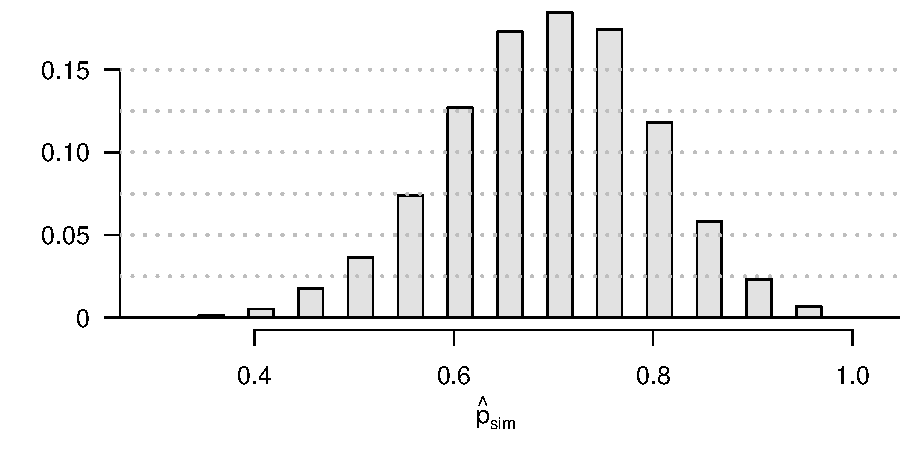
\includegraphics[width=0.8\textwidth]{ch_inference_for_props/figures/eoce/egypt/egypt}
\end{center}

\end{parts}
}{}

\textC{\newpage}

% 54

\eoce{\qt{Assisted Reproduction} Assisted Reproductive Technology (ART) is a collection of techniques that help facilitate pregnancy (e.g. in vitro fertilization). A 2008 report by the Centers for Disease Control and Prevention estimated that ART has been successful in leading to a live birth in 31\% of cases \footfullcite{web:art}. A new fertility clinic claims that their success rate is higher than average. A random sample of 30 of their patients yielded a success rate of 40\%. A consumer watchdog group would like to determine if this provides strong evidence to support the company's claim.
\begin{parts}
\item Write the hypotheses to test if the success rate for ART at this clinic is significantly higher than the success rate reported by the CDC.
\item Based on large sample theory, we modeled $\hat{p}$ using the normal distribution. Why is this not appropriate here?
\item The normal approximation would be less reliable here, so we should use a simulation strategy. Describe a setup for a simulation that would be appropriate in this situation and how the p-value can be calculated using the simulation results.
\item Below is a histogram showing the distribution of $\hat{p}_{sim}$ in 10,000 simulations under the null hypothesis. Estimate the p-value using the plot and use it to evaluate the hypotheses.
\item After performing this analysis, the consumer group releases the following news headline: ``Infertility clinic falsely advertises better success rates". Comment on the appropriateness of this statement.
\begin{center}
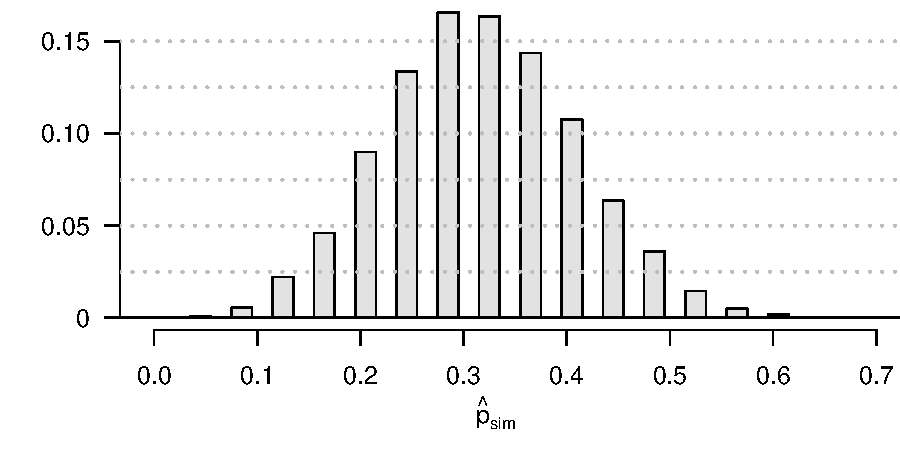
\includegraphics[width=0.85\textwidth]{ch_inference_for_props/figures/eoce/art/art}
\end{center}
\end{parts}
}{}

\textC{\newpage}


%__________________
\subsection{Randomization text (special topic)}

% 55

\eoce{\qt{Social experiment, Part II} Exercise~\ref{socExp} introduces a ``social experiment" conducted by a TV program that questioned what people do when they see a very obviously bruised woman getting picked on by her boyfriend. On two different occasions at the same restaurant, the same couple was depicted. In one scenario the woman was dressed ``provocatively" and in the other scenario the woman was dressed ``conservatively". The table below shows how many restaurant diners were present under each scenario, and whether or not they intervened.
\begin{center}
\begin{tabular}{ll cc c} 
            &               & \multicolumn{2}{c}{\textit{Scenario}} \\
\cline{3-4}
                            &           & Provocative   & Conservative  & Total \\
\cline{2-5}
\multirow{2}{*}{\textit{Intervene}} &Yes        & 5     & 15        & 20    \\
                            &No         & 15        & 10        & 25 \\
\cline{2-5}
                            &Total      & 20        & 25        & 45 \\
\end{tabular}
\end{center}
A simulation was conducted to test if people react differently under the two scenarios. 10,000 simulated differences were generated to construct the null distribution shown. The value $\hat{p}_{pr, sim}$ represents the proportion of diners who intervened in the simulation for the provocatively dressed woman, and $\hat{p}_{con, sim}$ is the proportion for the conservatively dressed woman.
\begin{center}
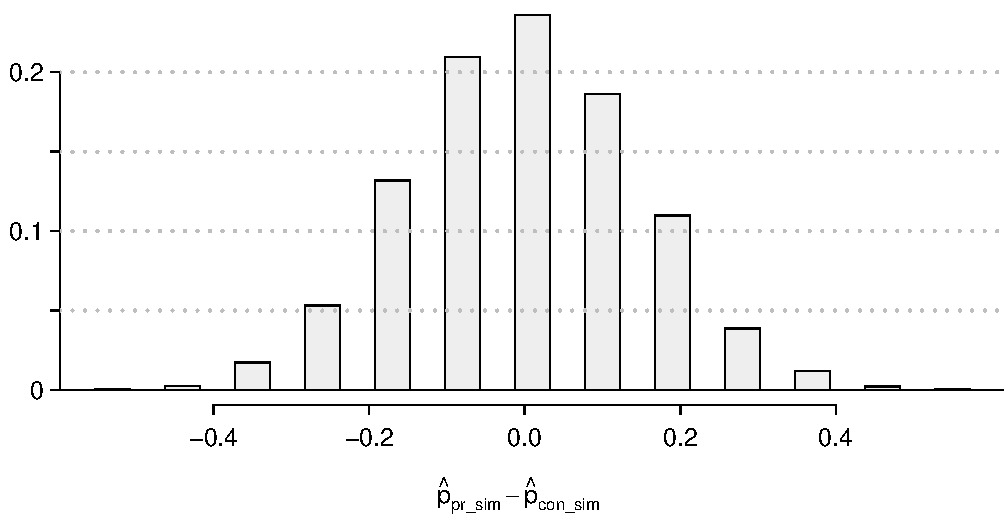
\includegraphics[width=0.9\textwidth]{ch_inference_for_props/figures/eoce/socExp/socExp}
\end{center}
\begin{parts}
\item What are the hypotheses? For the purposes of this exercise, you may assume that each observed person at the restaurant behaved independently, though we would want to evaluate this assumption more rigorously if we were reporting these results.
\item Calculate the observed difference between the rates of intervention under the provocative and conservative scenarios: $\hat{p}_{pr} - \hat{p}_{con}$.
\item Estimate the p-value using the figure above and determine the conclusion of the hypothesis test.
\end{parts}
}{}

\textC{\newpage}

% 56

\eoce{\qtq{Is yawning contagious} An experiment conducted by the \textit{MythBusters}, a science entertainment TV program on the Discovery Channel, tested if a person can be subconsciously influenced into yawning if another person near them yawns. 50 people were randomly assigned to two groups: 34 to a group where a person near them yawned (treatment) and 16 to a group where there wasn't a person yawning near them (control). The following table shows the results of this experiment. \footfullcite{data:yawn}
\begin{center}
\begin{tabular}{ll cc c} 
            &               & \multicolumn{2}{c}{\textit{Group}} \\
\cline{3-4}
                            &           & Treatment & Control   & Total \\
\cline{2-5}
\multirow{2}{*}{\textit{Result}}        &Yawn       & 10        & 4     & 14    \\
                            &Not Yawn   & 24        & 12        & 36 \\
\cline{2-5}
                            &Total      & 34        & 16        & 50 \\
\end{tabular}
\end{center}
A simulation was conducted to understand the distribution of the test statistic under the assumption of independence: having someone yawn near another person has no influence on if the other person will yawn. In order to conduct the simulation, a researcher wrote yawn on 14 index cards and not yawn on 36 index cards to indicate whether or not a person yawned. Then he shuffled the cards and dealt them into two groups of size 34 and 16 for treatment and control, respectively. He counted how many participants in each simulated group yawned in an apparent response to a nearby yawning person, and calculated the difference between the simulated proportions of yawning as $\hat{p}_{trtmt,sim} - \hat{p}_{ctrl,sim}$. This simulation was repeated 10,000 times using software to obtain 10,000 differences that are due to chance alone. The histogram shows the distribution of the simulated differences.
\begin{center}
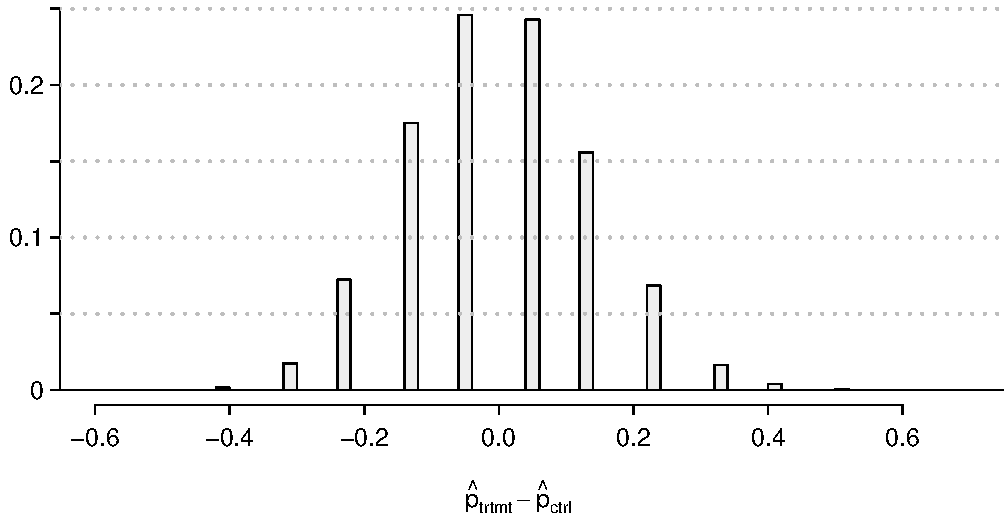
\includegraphics[width=0.9\textwidth]{ch_inference_for_props/figures/eoce/yawn/yawn}
\end{center}

\begin{parts}
\item What are the hypotheses?
\item Calculate the observed difference between the yawning rates under the two scenarios.
\item Estimate the p-value using the figure above and determine the conclusion of the hypothesis test.
\end{parts}
}{}

